\documentclass[journal]{IEEEtran}

% Packages
\usepackage{cite}
\usepackage{graphicx}
\usepackage{float}
\usepackage{stfloats}
\usepackage{amsmath, amssymb}

\begin{document}

% Title
\title{The quantum efficiency of hot-carrier generation in plasmonic nanoresonators}

% Author Information
\author{Wenqi Ji
\thanks{Wenqi Ji is with Department of Electrical and Computer Engineering, Rice University, Houston, USA (email: wj28@rice.edu).}
}

% Make title
\maketitle

% Abstract
\begin{abstract}
Conventional photocatalysts suffer from poor light absorption and inefficient hot carrier generation. Plasmonic antenna-reactor complexes overcome this problem by exploiting plasmonic resonances in metallic nanoparticles to enhance light collection and thereby enhance its absorption in the reactor nanoparticle. The absorbed photons produce energetic carriers in the reactor that catalyze the reaction. Optimizing these plasmonic antenna-reactor complexes for high absorption and highly efficient hot-carrier generation is an important step toward practical applications of plasmonic antenna-reactor photocatalysts. This project aims to rationally choose different metallic materials and geometries of plasmonic antenna-reactor complexes for any application. We use numerical simulations to optimize the materials and geometry and calculate the internal quantum efficiency of the plasmonic antenna-reactor complexes. We aim to design an antenna-reactor complex with nearly 100\% absorption in the specified bandwidth and achieve nearly 100\% internal quantum efficiency.
\end{abstract}

% Introduction
\section{Introduction}
\indent
Photocatalysts play a critical role in facilitating chemical reactions by converting optical energy into chemical energy. Conventional metal catalysts are often composed of transition-metal nanoparticles, which possess a favorable electronic structure that allows a variety of molecules to adsorb and react on their surfaces. Certain transition-metal nanoparticles can also harvest light through localized surface plasmon resonance (LSPR) and convert photon energy into energetic, non-equilibrium hot carriers. These hot carriers can directly participate in redox reactions or transfer into adsorbed molecules, thereby enabling light-driven chemical transformations. Such systems have demonstrated promising quantum efficiencies and favorable reaction selectivities compared to purely thermally driven processes\cite{doi:10.1021/nl502571b, https://doi.org/10.1002/anie.201308145}. However, their overall catalytic performance is often limited by inherently weak light–matter interactions\cite{10.1063/1.2734550}. Plasmonic metals such as Au, Ag, and Al, on the other hand, exhibit strong light–matter interactions due to their well-defined LSPR characteristics, but they typically lack intrinsic catalytic activity for many important chemical transformations\cite{doi:10.1021/acs.nanolett.6b03582}.\\
\indent
To address this limitation, a strategy was first proposed in Ref.~\cite{doi:10.1021/acs.nanolett.6b03582}, which integrates catalytically active metals with plasmonic metals such as Au, Ag, and Al. These plasmonic materials exhibit large optical cross-sections, support strong surface plasmon resonances, and significantly enhance the local electromagnetic fields. As a result, the generation of hot carriers within the catalytic metal components is substantially facilitated through near-field coupling. This approach enables the construction of strongly coupled plasmonic antenna–reactor systems, which offer enhanced optical absorption, accelerated reaction rates, and improved product selectivity across a broader range of reactions compared to their monometallic counterparts~\cite{https://doi.org/10.1002/advs.202302568}.\\
\indent
Specifically, Al–Pd nanodisk heterodimers were developed as antenna–reactor complexes, where the plasmonic Al component serves as the light-harvesting antenna and the Pd component functions as the catalytic reaction site~\cite{doi:10.1021/acs.nanolett.6b03582}.\\
\indent
Currently, plasmonic antenna-reactor systems typically adopt three distinct geometries, which are heterodimer, core–shell, and alloyed nanoparticle systems as shown in Figure \ref{fig:structure}\cite{https://doi.org/10.1002/advs.202302568}.\\
\indent
These structures have different advantages when applied to photocatalysis. The heterodimer structure is the easiest one to characterize and control the optical properties. Meanwhile, the broad optical response of both core-shell nanoparticles and the combination of different particle shapes aligns better with the solar spectrum than Pd nanoparticles alone\cite{Sytwu01012019}. \\
\indent
However, although plasmonic antenna-reactor systems can achieve high absorption, it's still not sufficient to guarantee effective catalytic performance. It is also crucial to ensure that most of the absorption occurs in the reactor nanoparticles, necessitating a high internal quantum efficiency (IQE) in the antenna-reactor system.\\
\indent
These plasmonic antenna-reactor systems quite suffer from low quantum efficiencies now, with the subsequent conversion of photons to reaction products quantified at no more than 2\% for various reactions under room temperature, despite high absorption\cite{Sytwu01012019}. Hence, we aim to achieve a plasmonic antenna-reactor photocatalyst design with near 100\% absorption internal quantum efficiency in the specified bandwidth.\\
\indent
In this work, we employ the finite-difference time-domain (FDTD) method to evaluate the optical performance, specifically the absorption and internal quantum efficiency (IQE) of three different antenna–reactor photocatalyst structures, including the heterodimer structure, the core–shell structure, and a newly proposed multi-layer structure, in order to identify the optimal configuration for broadband light harvesting.\\
\begin{figure}[H]
\centering
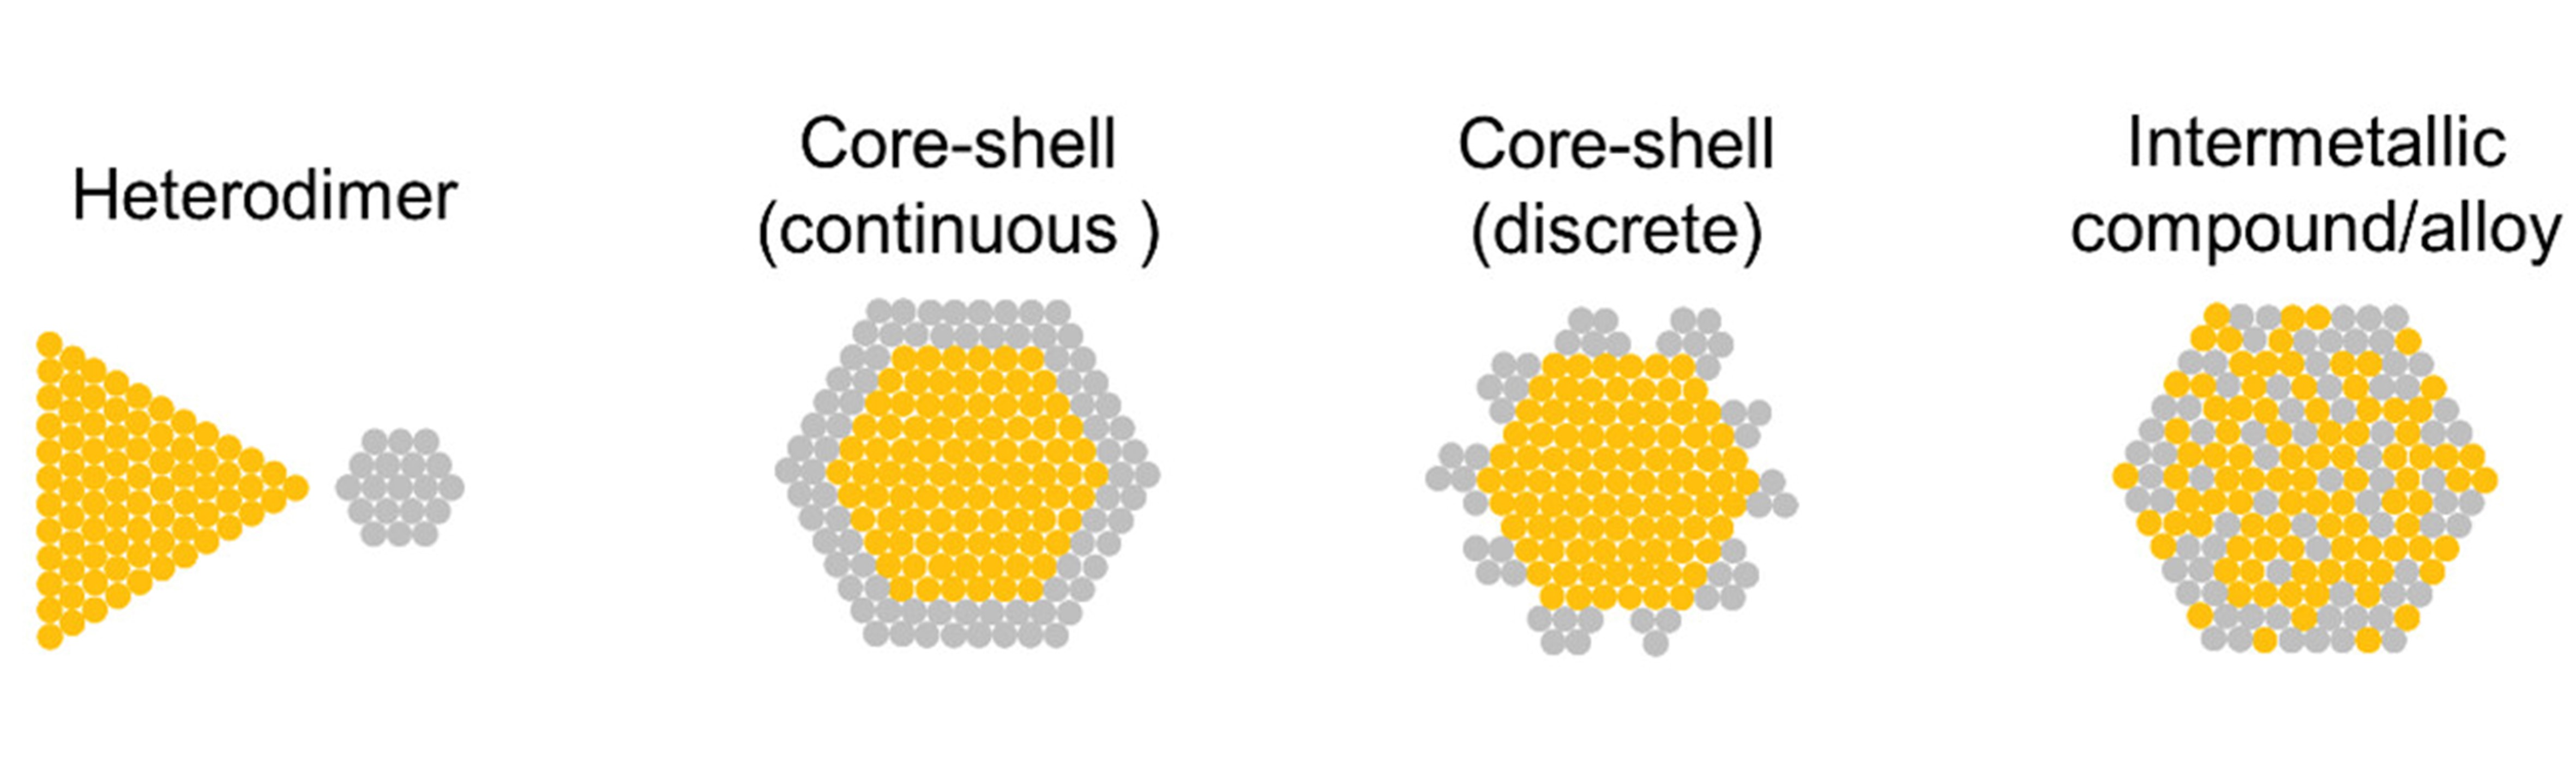
\includegraphics[width=80mm]{structure.jpg}
\caption{Three commonly used structures for antenna-reactor systems\cite{https://doi.org/10.1002/advs.202302568}.} 
\label{fig:structure} 
\end{figure}
% Methods
\section{Methods}
We use Lumerical FDTD to do the numerical simulation.\\
\indent
Here, we select a downward-propagating plane wave light source with the electric field polarized along the positive x-axis. The plane wave light source covers the wavelength from 400nm to 1000nm, positioned at a fixed height of 625 nm above the top surface of the substrate.  The reflection and transmission monitors are positioned 200 nm above the plane wave light source and 775 nm below the top surface of the substrate, respectively, with the latter monitor located inside the SiO$_2$ substrate.\\
\indent
The plane wave light source and monitors are set to cover the whole FDTD simulation region. The simulation region is set to be periodic in both the x-axis and y-axis directions with the same period length.\\
\indent
Since we use a plane wave light source, the scattering effects do not need to be considered. The total absorption can be directly calculated from reflectance and transmittance.\\
\begin{equation}
A_{total}=1-T_{total}-R_{total}
\label{eq:absorption}
\end{equation}
\indent
Power-absorbed (advanced) analysis groups are obtained for parts of different materials. The Pd absorption can then be determined by\\
\indent
\begin{equation}
A_{Pd} = A_{total} \times \frac{P_{Pd}}{P_{total}}
\label{eq:abspd}
\end{equation}
\indent
Where the total absorbed power is simply the sum of the absorbed power from all materials.\\
\indent
Pd, Al, and SiO$_2$ optical constants were obtained from Palik. TiO$_2$ optical constant was obtained from Siefke. Si optical constant was obtained from laboratory measurement.\\
% Results
\section{Results}
\indent
Heterodimer systems are widely utilized in photocatalysis primarily because plasmonic metals can support the collective resonant oscillation of free charge carriers near their surfaces, a phenomenon known as localized surface plasmon resonance (LSPR). This resonance gives rise to a highly enhanced, localized electromagnetic field that peaks at the metal surface and decays exponentially with distance. The intensified local field significantly boosts light absorption in adjacent catalytic nanoparticles, thereby improving photocatalytic efficiency.\\
\indent
We begin by simulating a basic heterodimer structure composed of Pd and Al cylinders, and systematically vary the layout and dimensions of the two components to enhance the Pd absorption. The schematic of the heterodimer configuration is shown in Figure~\ref{fig:heterodimer}(a), where the Pd and Al cylinders are constrained to have equal heights due to limitations in practical synthesis techniques.\cite{doi:10.1021/acs.nanolett.6b03582}\\
\indent
We first fix the sizes of both types of cylinders, setting their radii at 25 nm and heights at 50 nm. We find that varying either the edge-to-edge distance (d) between the Pd and Al cylinders within a single period, or the gap between Pd and Al cylinders across adjacent periods, results in similar trends. Moreover, the Pd absorption peak is highest when the distance equals the gap. Based on this observation, we then sweep the distance and gap simultaneously while keeping them equal.We observe that typically, the Pd absorption peak decreases as the distance between the Pd and Al cylinders increases; however, at very small separations, the peak can slightly increase with increasing distance. While maintaining a 3 nm distance between the Pd and Al cylinders, the Pd absorption reaches its highest peak, as shown in Figure~\ref{fig:heterodimer} (b). Since, in reality, distances smaller than 3 nm are easier to achieve, we further sweep the distance in finer steps from 0 nm to 3 nm, as shown in Figure~\ref{fig:heterodimer} (c). Again, we find that the Pd absorption peak is highest when the distance equals 3 nm. This trend can be explained by the fact that the incident electric field promotes strong near-field coupling around the Pd cylinders when interacting with the Al, a commonly used plasmonic metal. However, when the distance between the plasmonic and catalytic metals becomes extremely small, quantum mechanical effects become significant. In particular, nonradiative quenching of excited states at the metal surface becomes dominant \cite{AN20192228}, while plasmon–dipole decoupling \cite{doi:10.1021/jacs.5b12704} and quantum tunneling across the narrow gap \cite{doi:10.1021/nl304078v} further suppress the localized field enhancement. These effects collectively diminish plasmonic enhancement, leading to reduced hot carrier generation efficiency and overall light absorption.\\
\indent
Then we keep the optimal layout for the heterodimer cylinder structure, and change the heights and radii of these cylinders separately, as shown in Figure~\ref{fig:heterodimer} (d), (e), and (f). We find that a smaller lateral size consistently leads to higher Pd absorption in this structure, while increasing the height of the cylinders results in a slight enhancement in Pd absorption. However, synthesizing nanocylinders with the heights around several hundred nanometers remains challenging in practical experimental settings.\\
\begin{figure}[H]
\centering
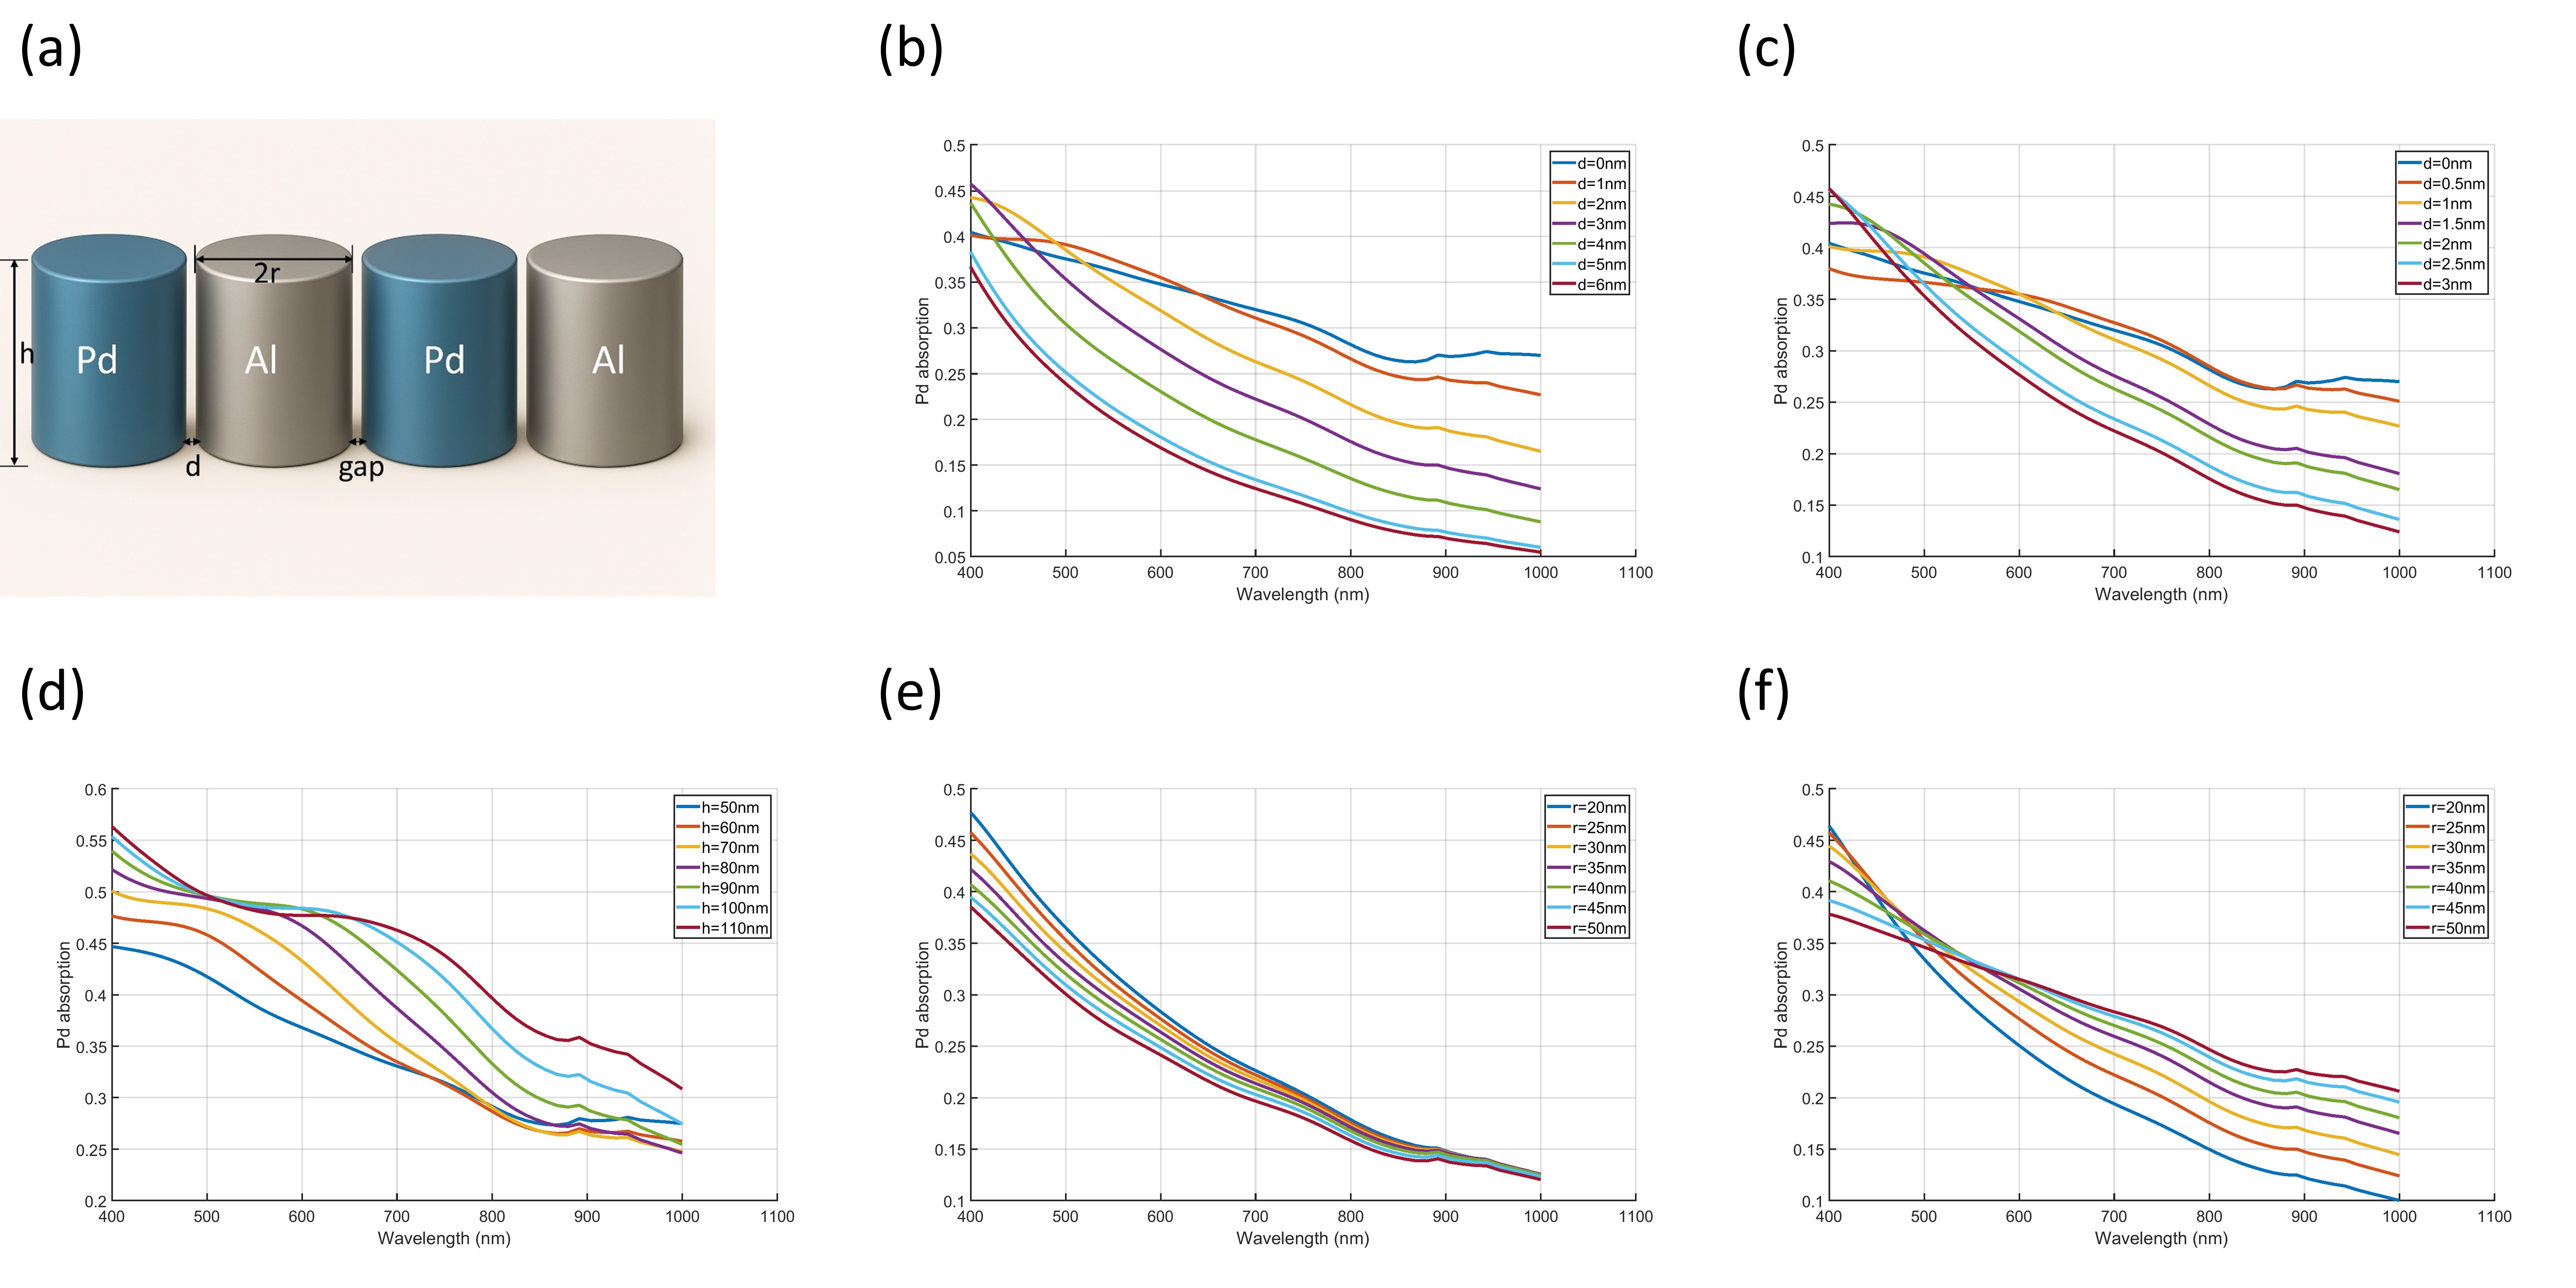
\includegraphics[width=80mm]{heterodimerstructure.jpg}
\caption{Heterodimer structure. (a) Schematic of the heterodimer structure across two periods. (b) Simultaneous variation of the edge-to-edge distance (d) and the gap between Pd and Al cylinders (r=25nm, h=50nm). (c) Simultaneous variation of the edge-to-edge distance (d) and the gap between Pd and Al cylinders with finer steps (r=25nm, h=50nm). (d) Simultaneous variation of the heights of both Pd and Al cylinders (r=25nm, d=gap=3nm). (e) Variation of the radius of Al cylinders only (r$_\text{Pd}$ =25nm, h=50nm, d=gap=3nm). (f) Simultaneous variation of the radii of both Pd and Al cylinders (h=50nm, d=gap=3nm).
} 
\label{fig:heterodimer} 
\end{figure}
\indent
Figure \ref{fig:Efield_heterodimer} shows the cross-sectional view of the electric field distribution in the x–z plane for a two-period heterodimer structure, highlighting the localized enhancement of the electric field and providing insight into the previously discussed trend in Pd absorption.\\
\begin{figure}[H]
\centering
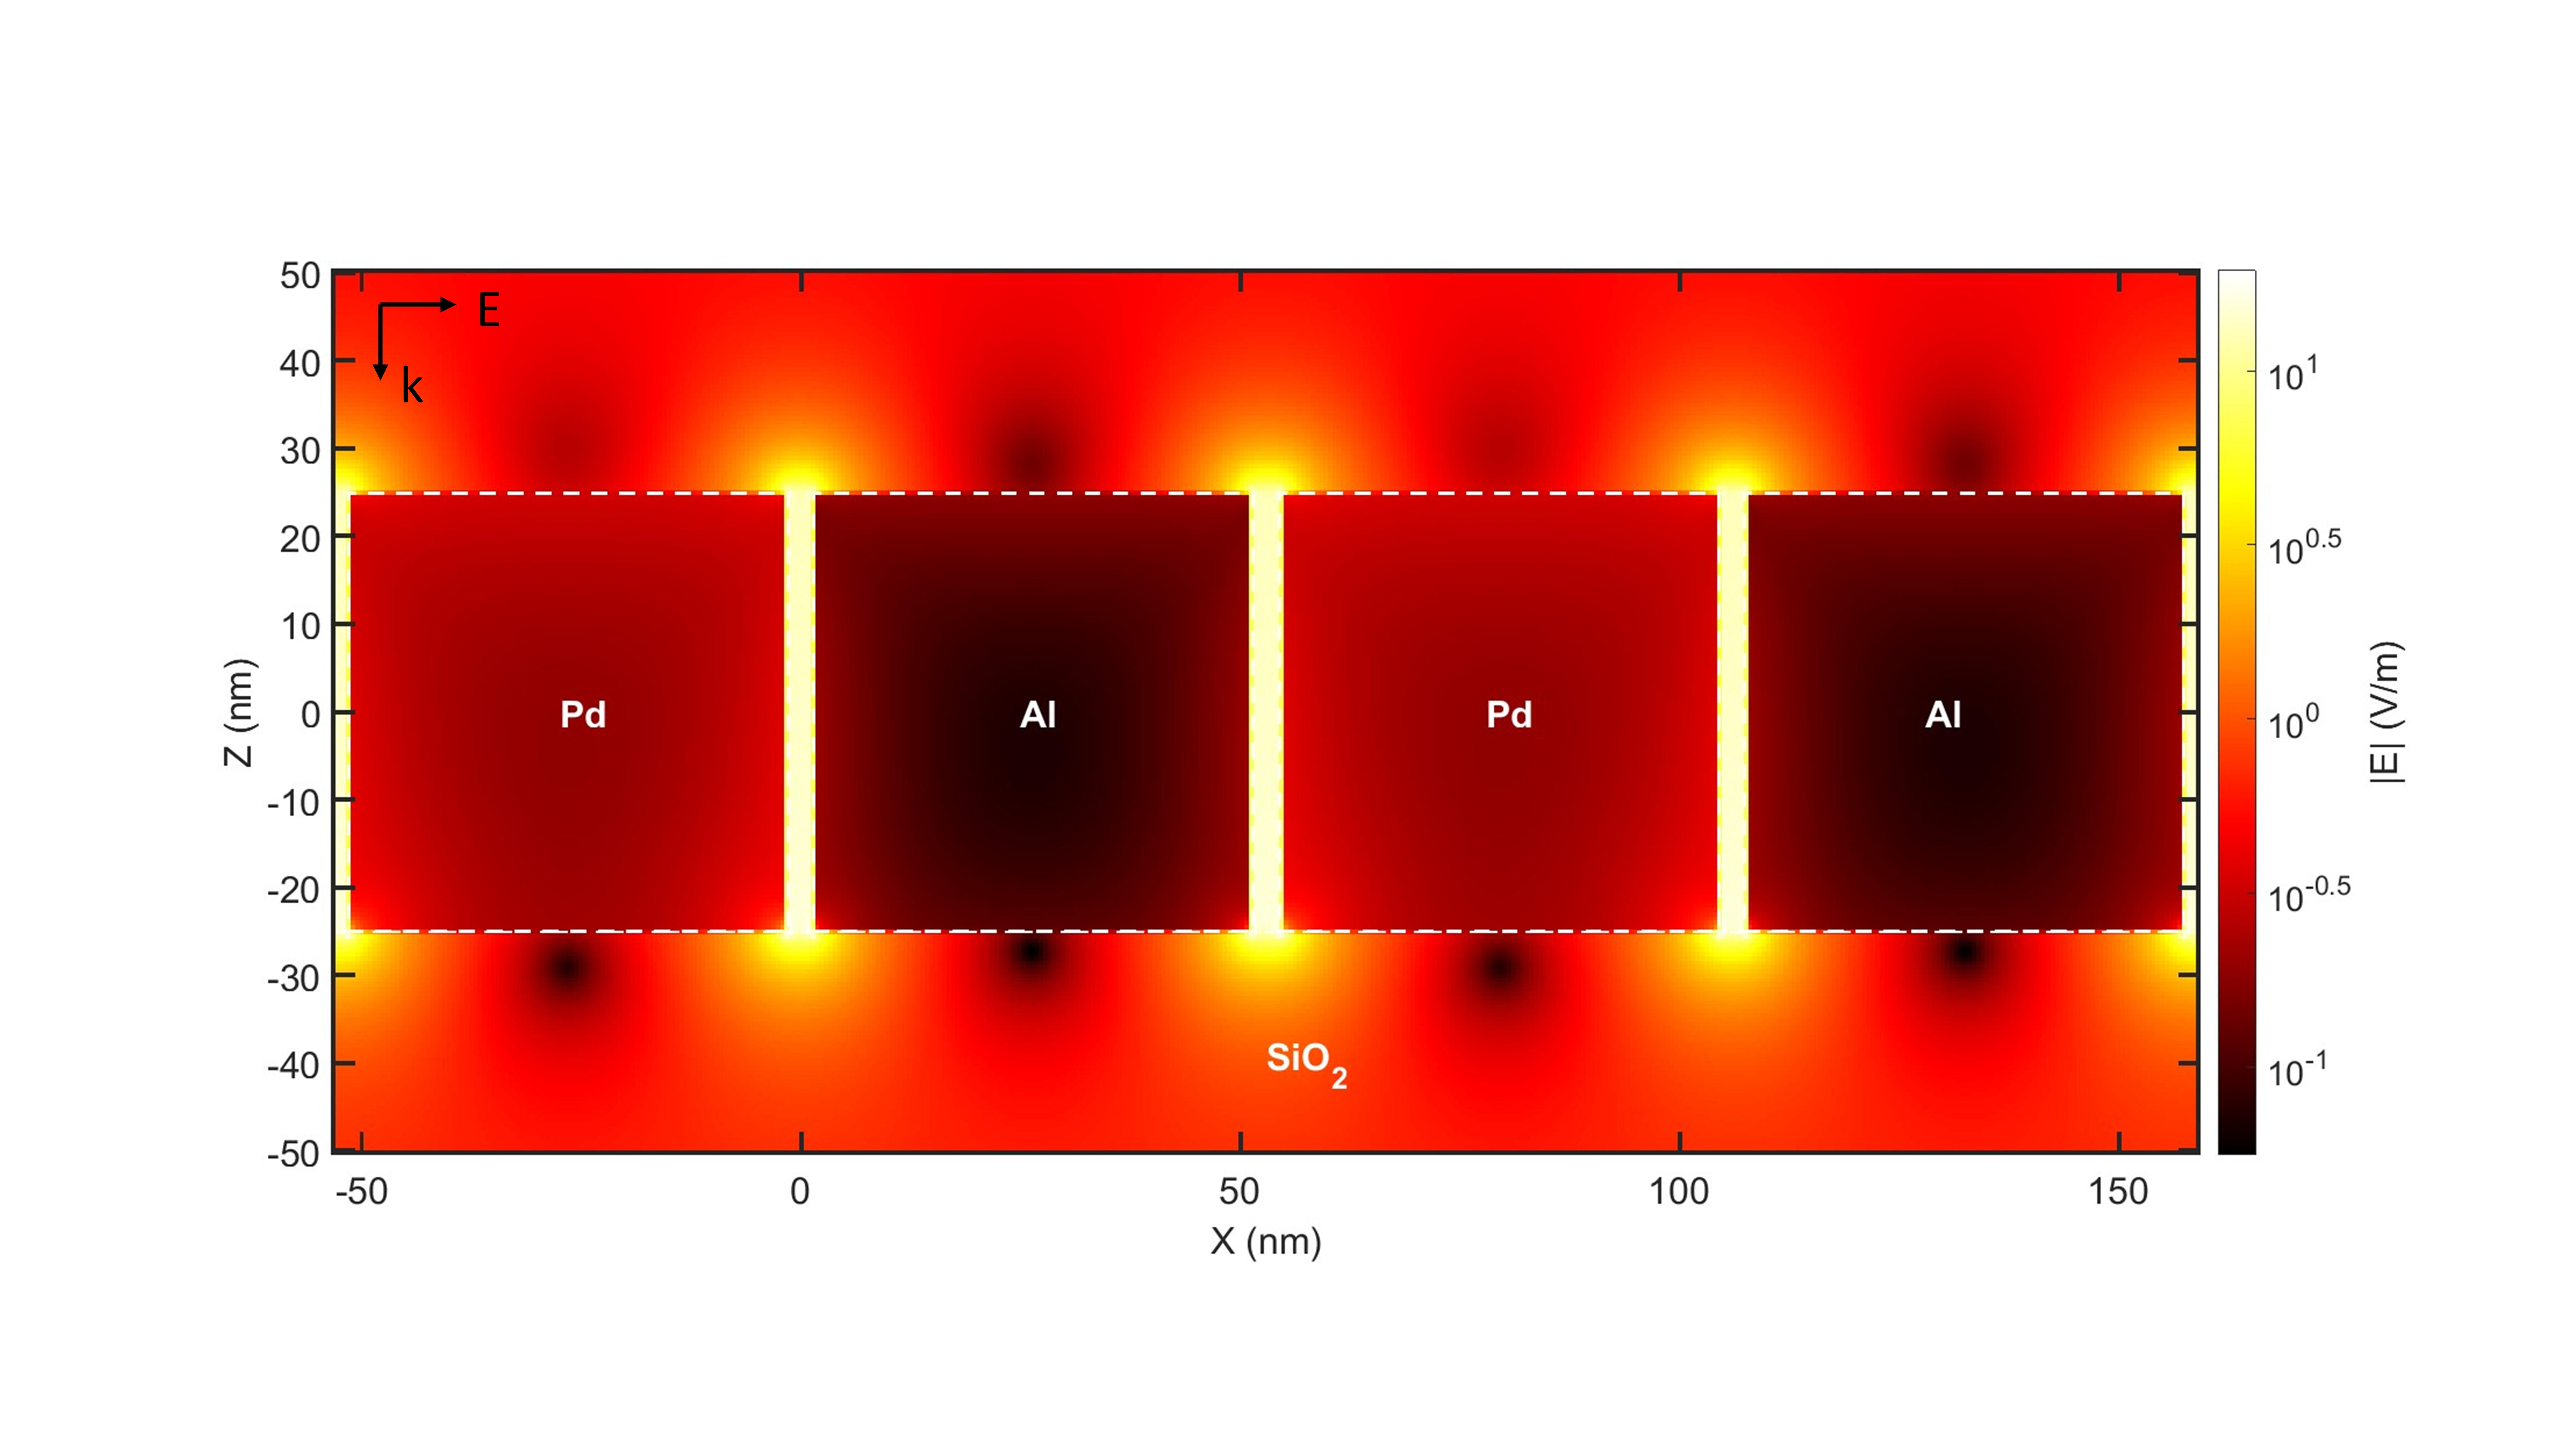
\includegraphics[width=80mm]{Efield_heterodimer.jpg}
\caption{Cross-sectional view of the electric field distribution in the x–z plane for a two-period heterodimer structure (r=25nm, h=50nm, d=gap=3nm. } 
\label{fig:Efield_heterodimer} 
\end{figure}
\indent
We propose a multi-layer antenna-reactor structure inspired by the Salisbury screen, which consists of catalytic Pd nanostructures on the top, a dielectric spacer layer, and a bottom metallic Al layer serving primarily as a reflective plane. In this configuration, Al does not support localized surface plasmon resonance (LSPR) due to its continuous film form and role as a mirror. In contrast, Pd, while not a conventional plasmonic metal, exhibits moderate plasmonic behavior. When structured at the nanoscale, Pd can support LSPR, leading to localized electric field enhancement near its surface, which in turn increases light absorption in the Pd layer and enhances hot carrier generation for photocatalytic applications.\\
\indent
We perform simulations using both Si and TiO$_2$ as the dielectric spacer layer, and ultimately select TiO$_2$. This choice is primarily due to its negligible imaginary part of the permittivity, $\operatorname{Im}[\epsilon]$\, which means minimal intrinsic absorption loss within the spacer itself. In contrast, Si exhibits significant absorption in the visible range, which can reduce the effective light intensity reaching the catalytic Pd layer. Furthermore, the use of TiO$_2$ enables a higher Pd absorption over a broader range of incident wavelengths compared to Si, benefiting from its high refractive index and low optical loss, which together facilitate more efficient interference-based field enhancement.\\
\indent
Additionally, for all the multi-layer structures studied, once the Al layer thickness reaches approximately 40 nm, further increases do not lead to significant improvements in Pd absorption. This is because the Al layer has already behaved as an almost perfect reflector at this thickness. Therefore, in the subsequent simulations, the Al layer is treated as a perfect reflector, and its thickness is fixed at 40 nm.\\
\indent
For multi-layer structures incorporating Pd cubes, Pd absorption increases with the size of the Pd nanostructures. In the case of Pd cylinders, a similar trend is observed as in heterodimer systems: Pd absorption increases as the cylinder radius decreases and the height increases. Figure \ref{fig:multi-layer cylinder and cube} presents the multi-layer configurations with Pd cubes and cylinders, and shows how Pd absorption changes with varying the distance between each Pd nanosructure and dielectric spacer thickness.\\
\indent
It can be seen that, within a limited range, increasing the gap distance between Pd nanostructures results in enhanced Pd absorption for both configurations, exhibiting a similar behavior to that observed in heterodimer cylinders.\\
\indent
Moreover, the shift of the Pd absorption peak with varying TiO$_2$ thickness is consistent with the behavior expected from the Salisbury screen model. However, we also observe that the peak absorption appears when the incident wavelength is slightly shorter than four times the product of the TiO$_2$ refractive index and its thickness (i.e., $\lambda < 4nt$). This deviation arises because the Salisbury screen represents an idealized case, whereas in our simulation, the Al layer is not a perfect reflector, and losses or phase shifts at the Al interface affect the interference condition.\\
\begin{figure}[H]
\centering
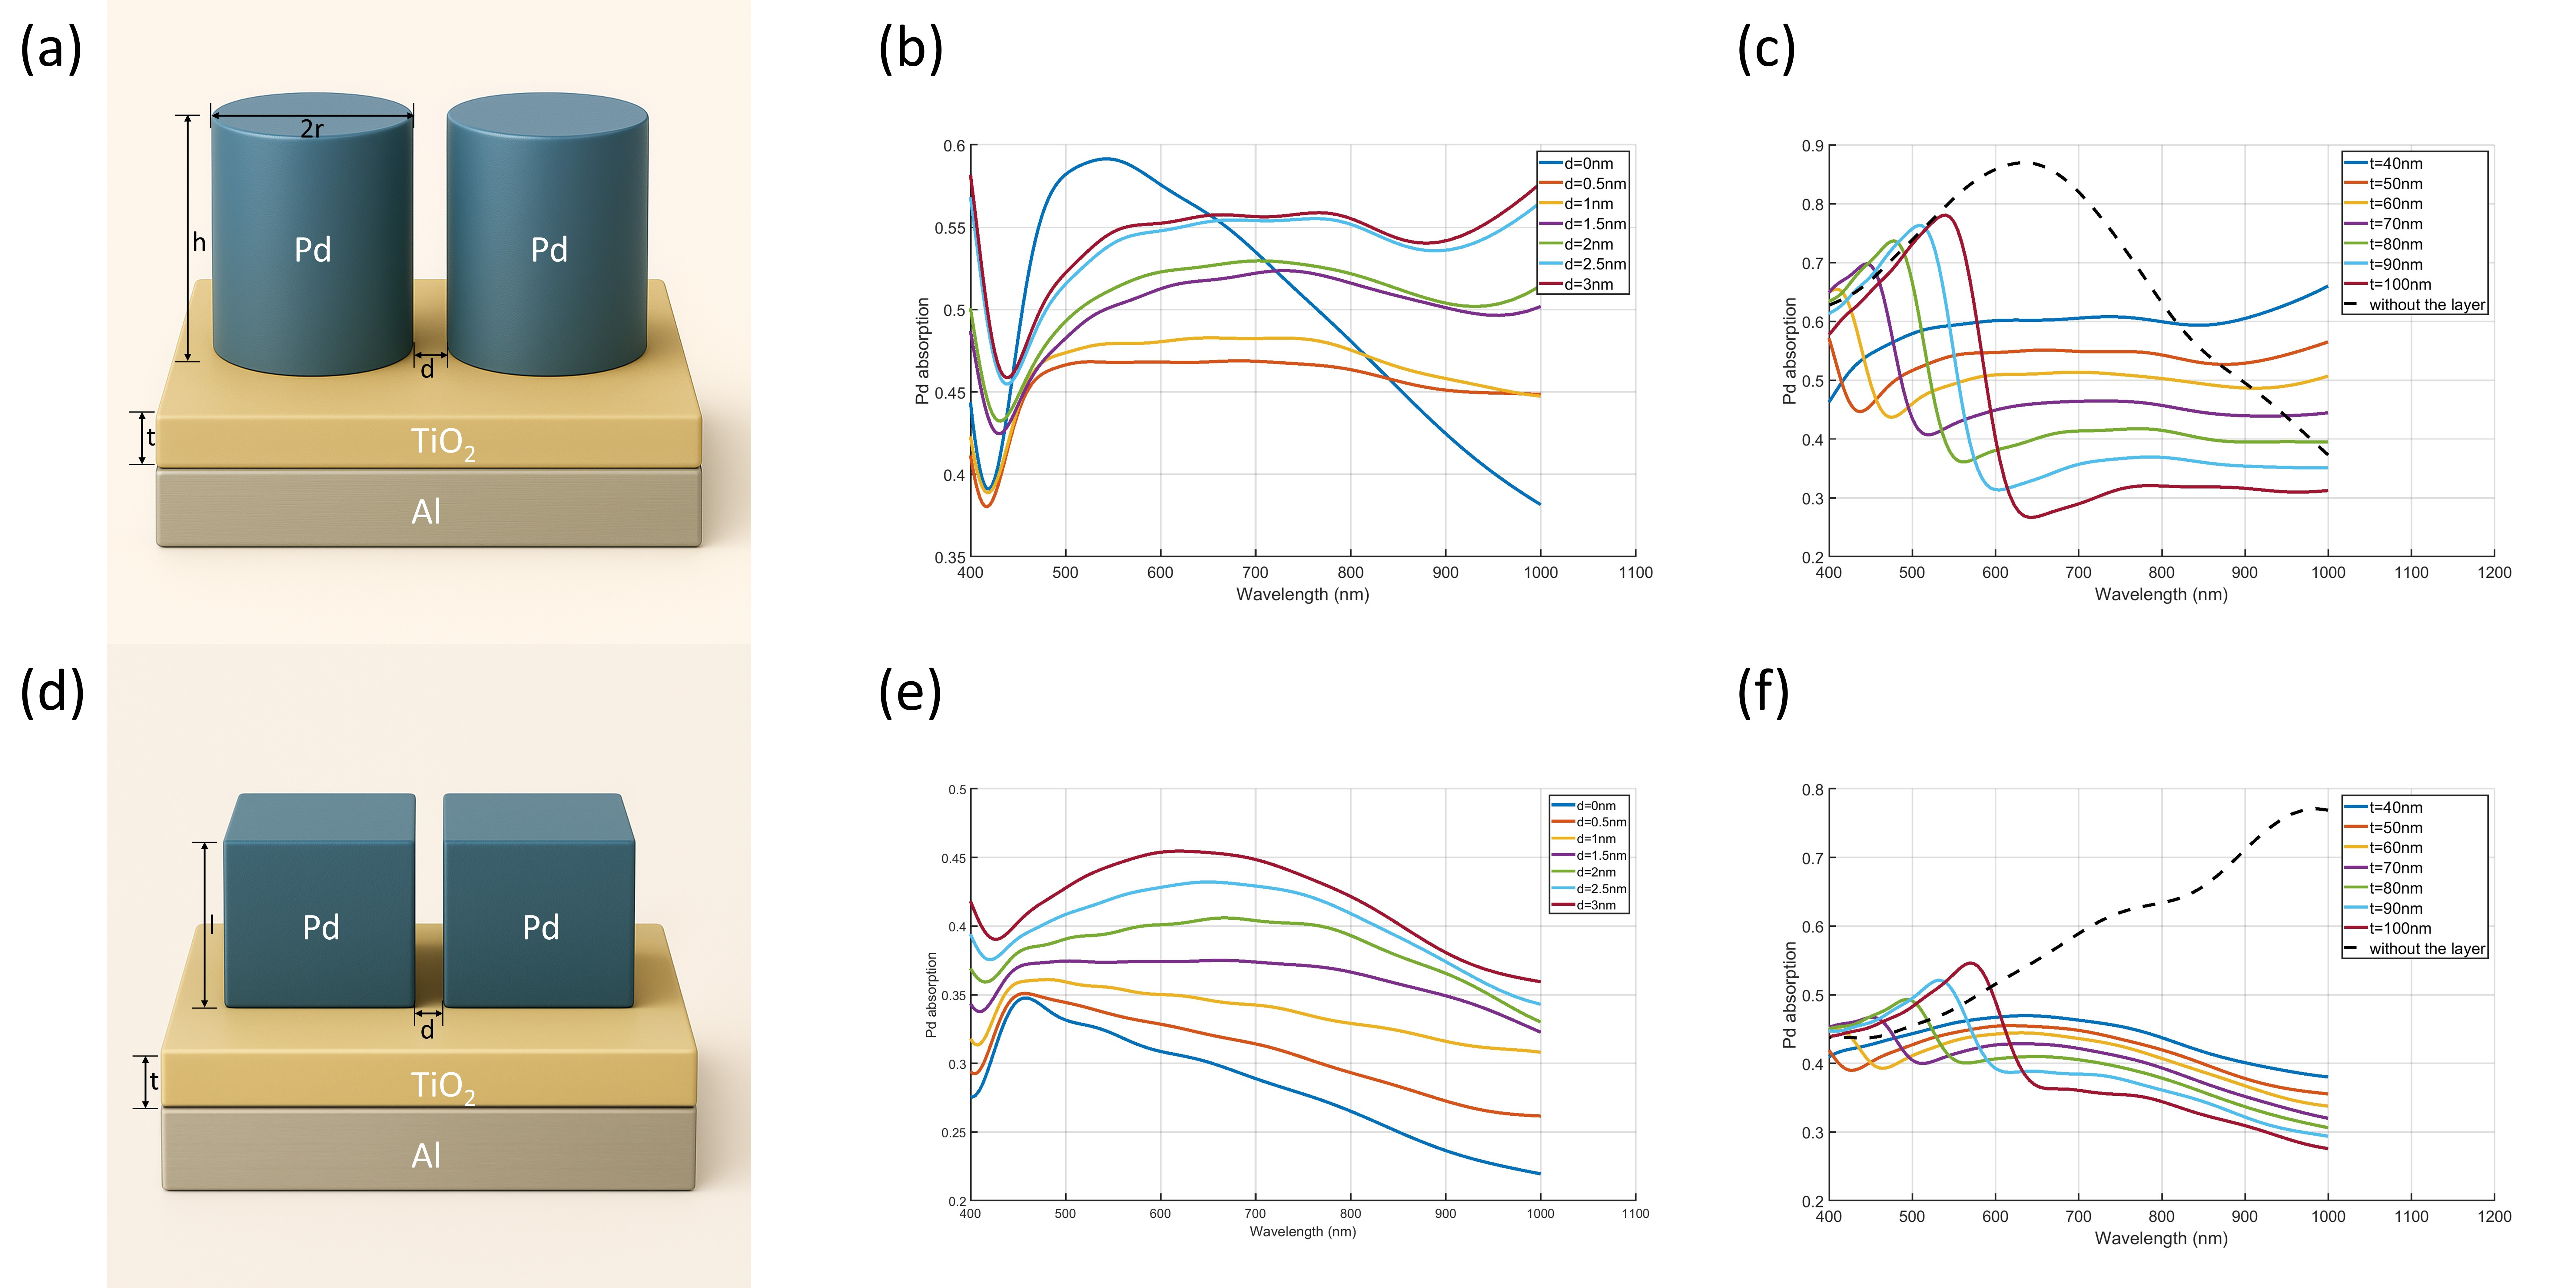
\includegraphics[width=80mm]{multi-layer_cube_cylinder.jpg}
\caption{Multi-layer structures. (a) Schematic of the multi-layer structure incorporating Pd cylinders. (b) Variation of the gap between Pd cylinders (r=25nm, h=50nm, t=50nm). (c)Variation of the TiO$_2$ thickness (r=25nm, h=50nm, d=3nm). (d) Schematic of the multi-layer structure incorporating Pd cubes. (b) Variation of the gap between Pd cubes (l=50nm, t=50nm). (c)Variation of the TiO$_2$ thickness (l=50nm, d=3nm).} 
\label{fig:multi-layer cylinder and cube} 
\end{figure}
\indent
For multi-layer structures incorporating Pd spheres, which behave quite differently from those with Pd cubes or cylinders, the highest Pd absorption is achieved when the adjacent Pd spheres are just in contact with each other. This is because Pd spheres rely on inter-particle plasmonic coupling rather than localized field enhancement at sharp corners or edges, due to their smooth and symmetric geometry, which inherently lacks strong local hotspots. Furthermore, because of this geometry, such multi-layer structures exhibit relatively consistent peak Pd absorption across different TiO$_2$ thicknesses, and interestingly, they show two distinct absorption peaks within the incident wavelength range of 400–1000 nm. Additionally, increasing the Pd sphere size leads to a red shift in the absorption peak wavelength, while the peak absorption magnitude remains nearly unchanged.\\
\indent
The multi-layer structure incorporating Pd spheres demonstrates strong potential as an effective photocatalyst system, as it can achieve a peak Pd absorption of approximately 90\% while maintaining broad spectral coverage across a wide range of incident wavelengths. Furthermore, the desired absorption wavelength can be easily tuned by adjusting the TiO$_2$ thickness, without compromising the overall Pd absorption efficiency.\\
\indent
To further evaluate the photocatalytic performance of this structure, we analyze the internal quantum efficiency (IQE) and the probability of chemical reaction, as shown in Figure~\ref{fig:multi-layer sphere}(e).\\
\indent
In this analysis, we assume that all absorbed photons contribute to the generation of hot carriers. Under this assumption, the internal quantum efficiency (IQE) is defined as the ratio of photons absorbed by the Pd to the total number of absorbed photons.\\
\indent
As shown in this figure, both IQE and Pd absorption generally follow a similar trend with incident wavelength. They initially decrease and form a small dip around 450 nm, then increase to reach a peak value, and afterwards show some fluctuations at longer wavelengths.\\
\indent
Additionally, we define the plasmonic enhancement rate in steady state as being proportional to the ratio of the number of newly generated hot carriers in Pd per unit volume and unit time to the number of hot carriers in thermal equilibrium. \\
\indent
\begin{equation}
    Rate_{\text{plasmonic enhancement}} \propto \frac{\Delta
    N_{\text{hot carriers}}}{N_0}
    \label{eq:probability}
\end{equation}
\indent
The steady-state condition here refers to the dynamic equilibrium between the generation and relaxation of hot carriers, where the rate of hot carrier relaxation equals the rate of photon absorption. Under this assumption, the number of non-equilibrium hot carriers, \( \Delta N \), generated in Pd can be expressed as:
\begin{equation}
\Delta N = R_{\text{abs}} \cdot \tau
\label{eq:deltaN}
\end{equation}
\indent
where \( R_{\text{abs}} \) is the photon absorption rate—defined as the number of photons absorbed per unit volume per unit time in the Pd region.  \( \tau \) is the carrier relaxation time.\\
\indent
The absorption rate can be further expressed as:
\begin{equation}
R_{\text{abs}} = \frac{P_{\text{Pd, abs}}}{\hbar \omega \cdot V_{\text{Pd}}}
\label{eq:Rabs}
\end{equation}
\indent
where \( P_{\text{Pd, abs}} \) denotes the total optical power absorbed in Pd, \( \hbar \omega \) is the photon energy, and \( V_{\text{Pd}} \) is the absorption volume of the Pd nanostructure.\\
\indent
In this context, the relaxation time \( \tau \) is calculated using the Drude model. Given that the Pd nanostructure is sufficiently small, the relaxation time obtained from the Drude model is assumed to reliably represent the actual hot carrier relaxation time.\\
\indent
Under thermal equilibrium, the total number of electrons with energies above the Fermi level \( E_F \) can be calculated by integrating the product of the density of states \( D(E) \) and the Fermi-Dirac distribution \( f(E, T) \) from \( E_F \) to infinity:
\begin{equation}
N_0 = \int_{E_F}^{\infty} D(E) \cdot f(E, T) \, dE
\label{eq:hot_electron_integral}
\end{equation}
\indent
Where the Fermi-Dirac distribution is defined as:
\begin{equation}
f(E, T) = \frac{1}{e^{(E - E_F)/k_B T} + 1}
\label{eq:fermi_dirac}
\end{equation}
\indent
Here, \( D(E) \) is the electronic density of states, which is assumed to be constant near the Fermi level: \( D(E) = 0.2~\mathrm{eV^{-1} \cdot m^{-3}} \). \( E_F \) is the Fermi level, \( k_B \) is the Boltzmann constant, and \( T \) is the absolute temperature, taken as room temperature: \( T = 295~\mathrm{K} \).\\
\indent
As shown in the plot, the chemical reaction probability also exhibits a dip around 450 nm. At longer wavelengths, the photon absorption rate increases, which in turn generates more hot carriers and consequently enhances the probability of chemical reactions after the dip.\\
\begin{figure}[H]
\centering
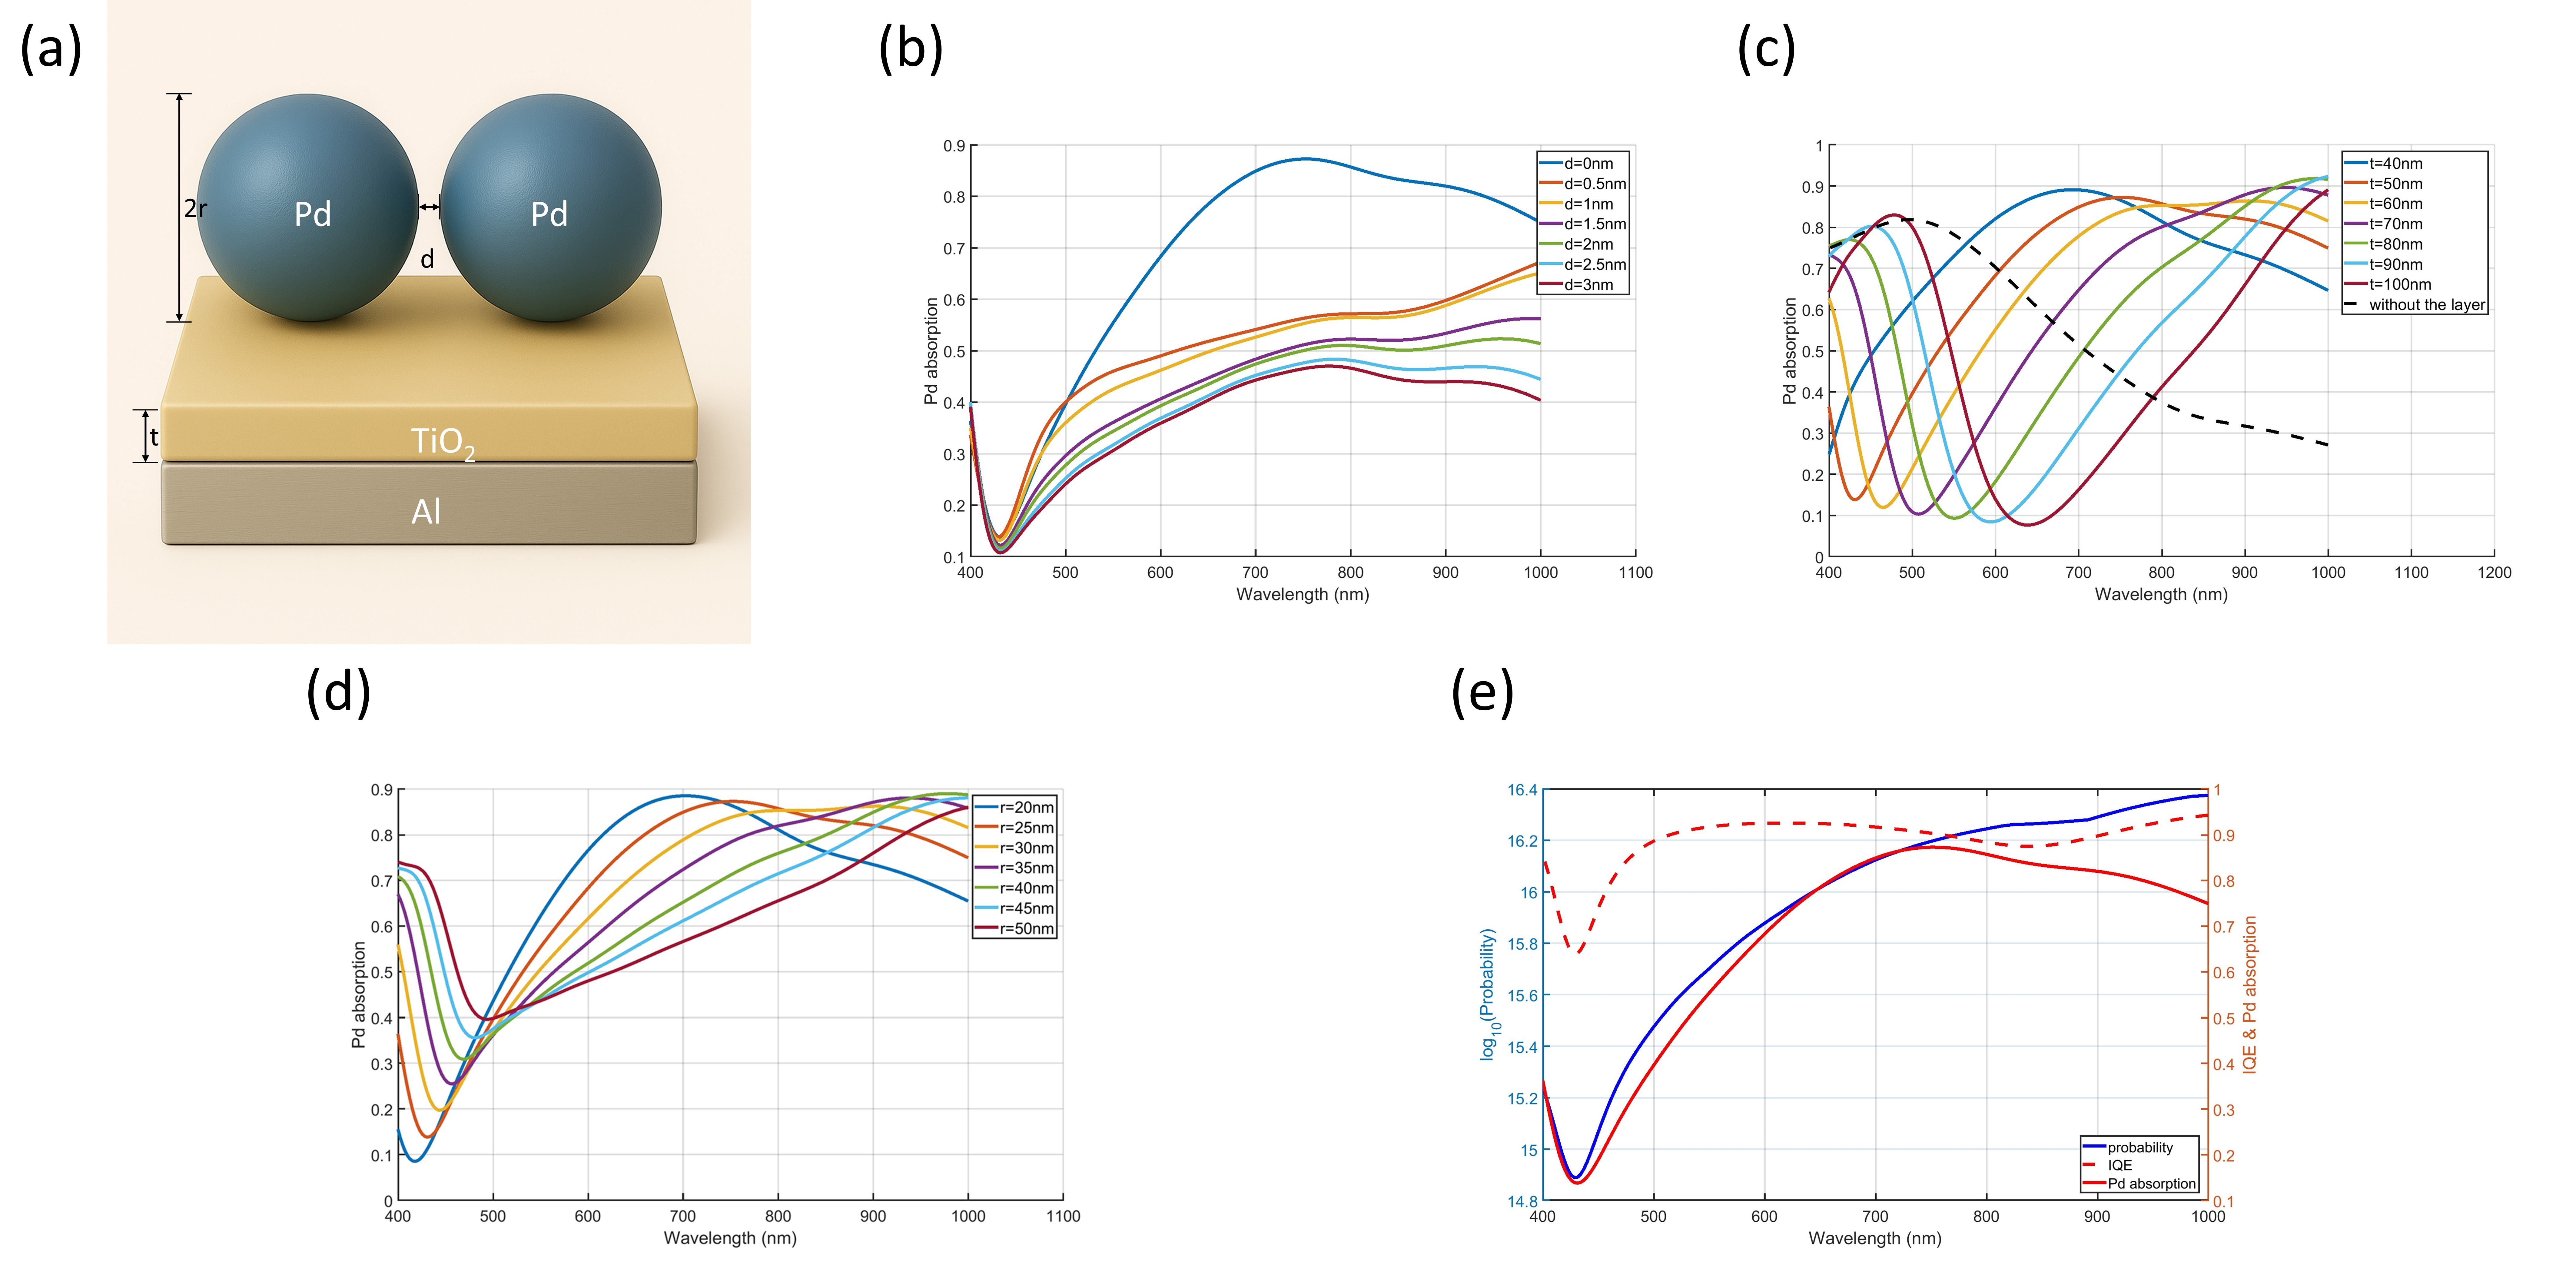
\includegraphics[width=80mm]{multi-layer_sphere.jpg}
\caption{Multi-layer structures incorporating Pd spheres. (a) Schematic of the multi-layer structure incorporating Pd spheres. (b) Variation of the gap between Pd spheres (r=25nm, t=50nm). (c) Variation of the TiO$_2$ thickness (r=25nm, d=0nm). (d) Variation of the radius of Pd sphere (t=50nm, d=0nm). (e) Plot of the internal quantum efficiency (IQE), Pd absorption, and the plasmonic enhancement rate (r=25nm, t=50nm, d=0nm).} 
\label{fig:multi-layer sphere} 
\end{figure}
\indent
Figure \ref{fig:Efield_multilayer} shows the cross-sectional view of the electric field distribution in the x–z plane for a two-period multi-layer structure. As shown in the figure, the Pd sphere structure exhibits the strongest localized electric field enhancement, indicating that it is the optimal design among the configurations considered. In contrast, the Pd cube structure at this size does not produce a significant electric field enhancement, resulting in the lowest Pd absorption among the tested geometries.\\
\begin{figure}[H]
\centering
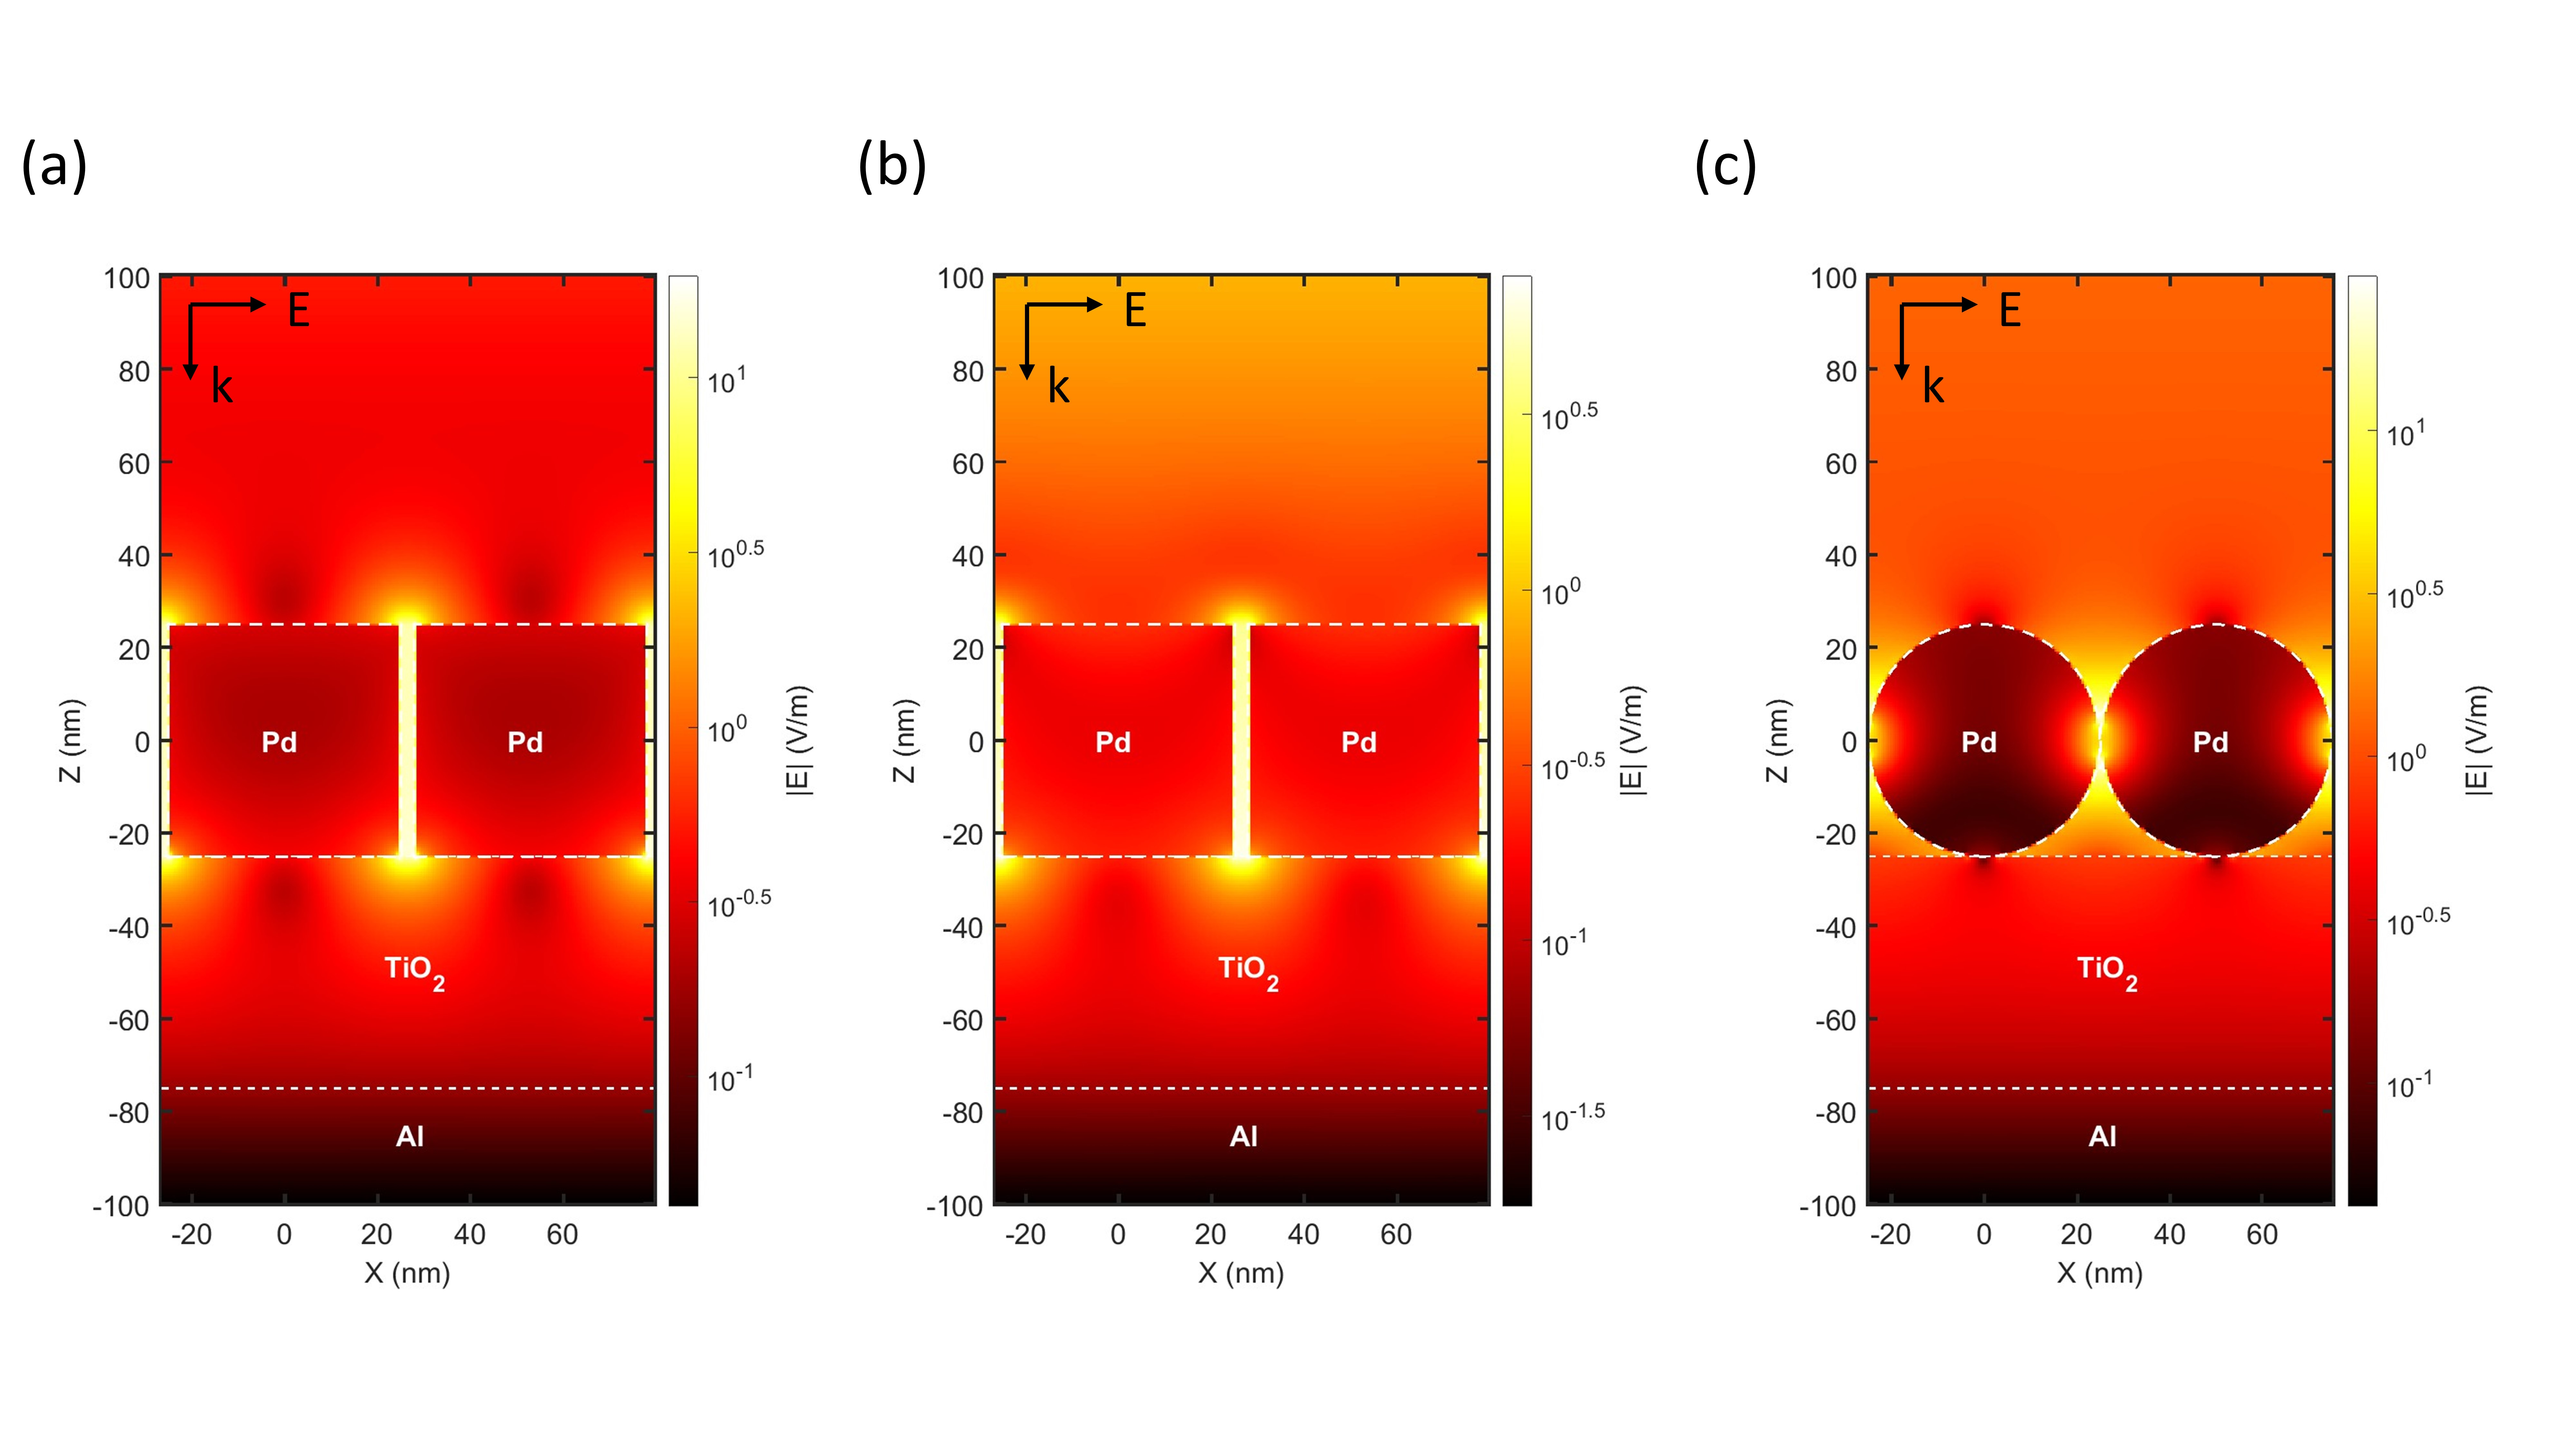
\includegraphics[width=80mm]{Efield_multilayer.jpg}
\caption{Cross-sectional view of the electric field distribution in the x–z plane for a two-period multi-layer structures. (a) Pd cylinders (r=25nm, h=50nm, t=50nm, d=3nm). (b) Pd cubes (l=50nm, t=50nm, d=3nm). (c) Pd spheres (r=25nm, t=50nm, d=0nm).} 
\label{fig:Efield_multilayer} 
\end{figure}
\indent
\indent
For core–shell structures, the mechanism of antenna–reactor systems used in photocatalysis differs slightly. Instead of relying primarily on hot carriers generated within the Pd nanoparticles to drive catalysis, this type of structure utilizes hot carriers generated in the Al core, which are rapidly transferred to the surrounding Pd shell where the catalytic reactions take place. This helps explain why, despite the enhancement of photocatalytic performance often observed in core–shell configurations, our simulations show that Pd absorption in such structures remains relatively low, even compared to structures composed solely of Pd.\\
\indent
The schematics of the core–shell cube and sphere structures, along with the corresponding variations in Pd absorption as a function of the distance between each cube and Al core size, are presented in Figure~\ref{fig:core-shell}. The trends in Pd absorption with respect to the distance are consistent with those observed in the multi-layer structures discussed earlier.\\
\begin{figure}[H]
\centering
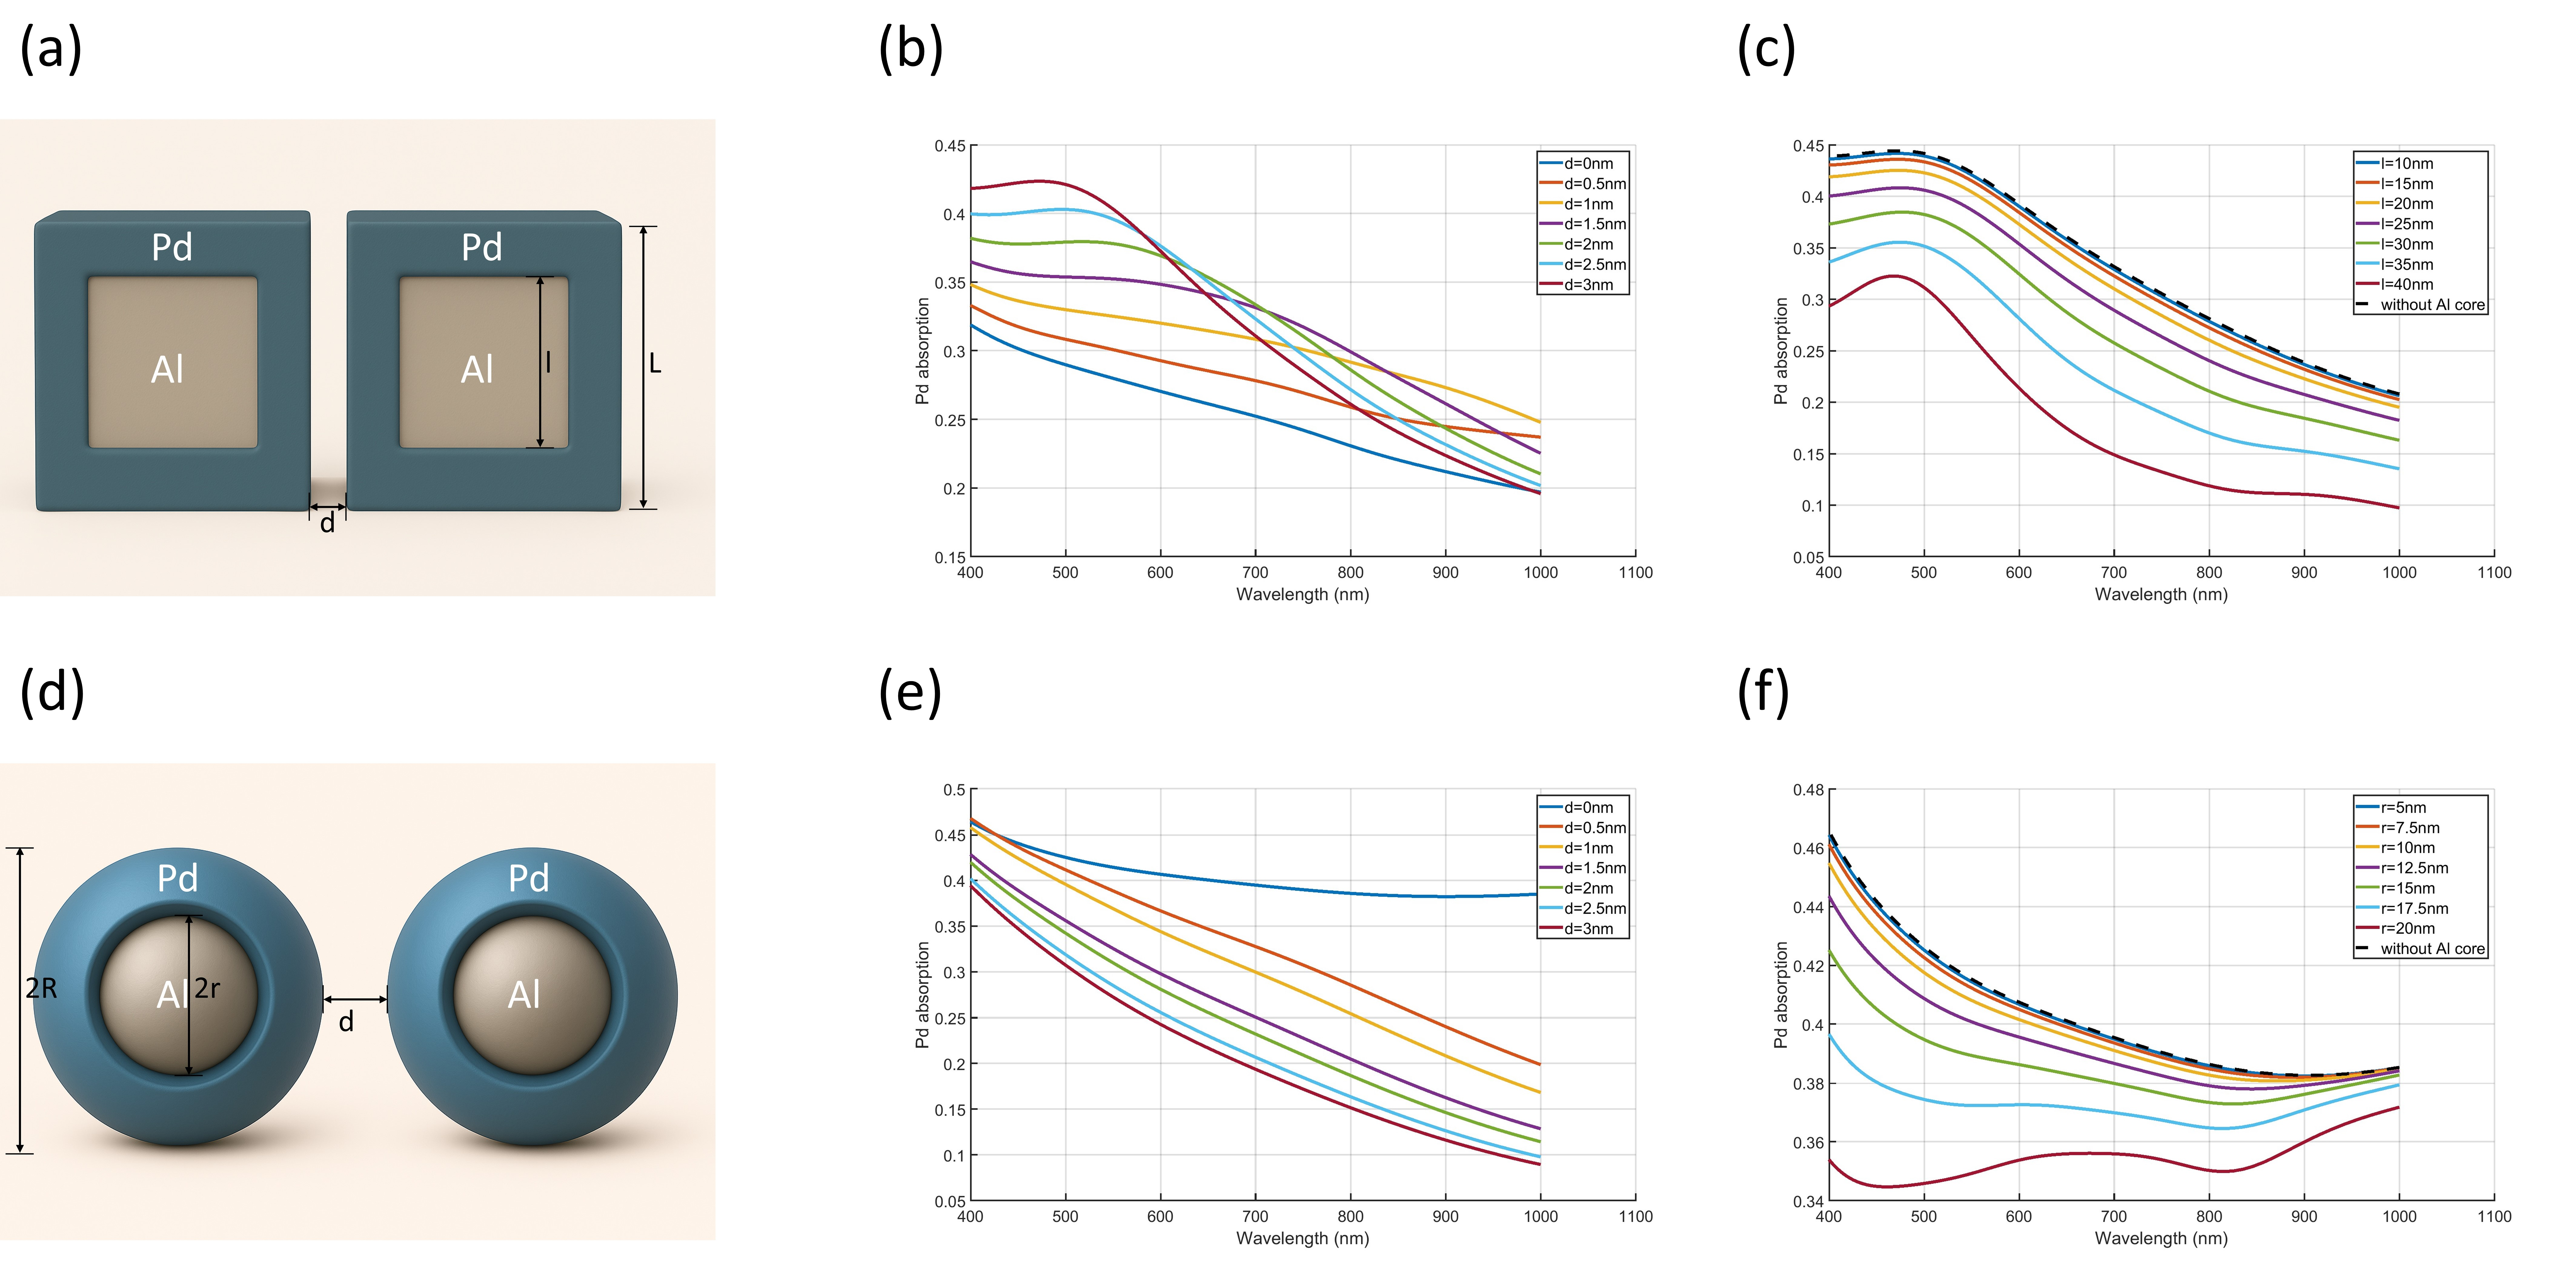
\includegraphics[width=80mm]{core-shellstructure.jpg}
\caption{Core-shell structure. (a) Schematic of the core-shell cube structure. (b) Variation of length of Al core (L=50nm, d=3nm). (c) Schematic of the core-shell sphere structure. (b) Variation of radius of Al core (R=25nm, d=0nm).} 
\label{fig:core-shell} 
\end{figure}
\indent
Figure \ref{fig:core-shell} shows the cross-sectional view of the electric field distribution in the x–z plane for a two-period core–shell structure. As illustrated, the Al cores do not significantly enhance the local electric field within the surrounding Pd shells, leading to limited Pd absorption. Additionally, consistent with the observations in the multi-layer structures, the sphere configurations generate stronger localized electric fields compared to the cube structures.\\
\begin{figure}[H]
\centering
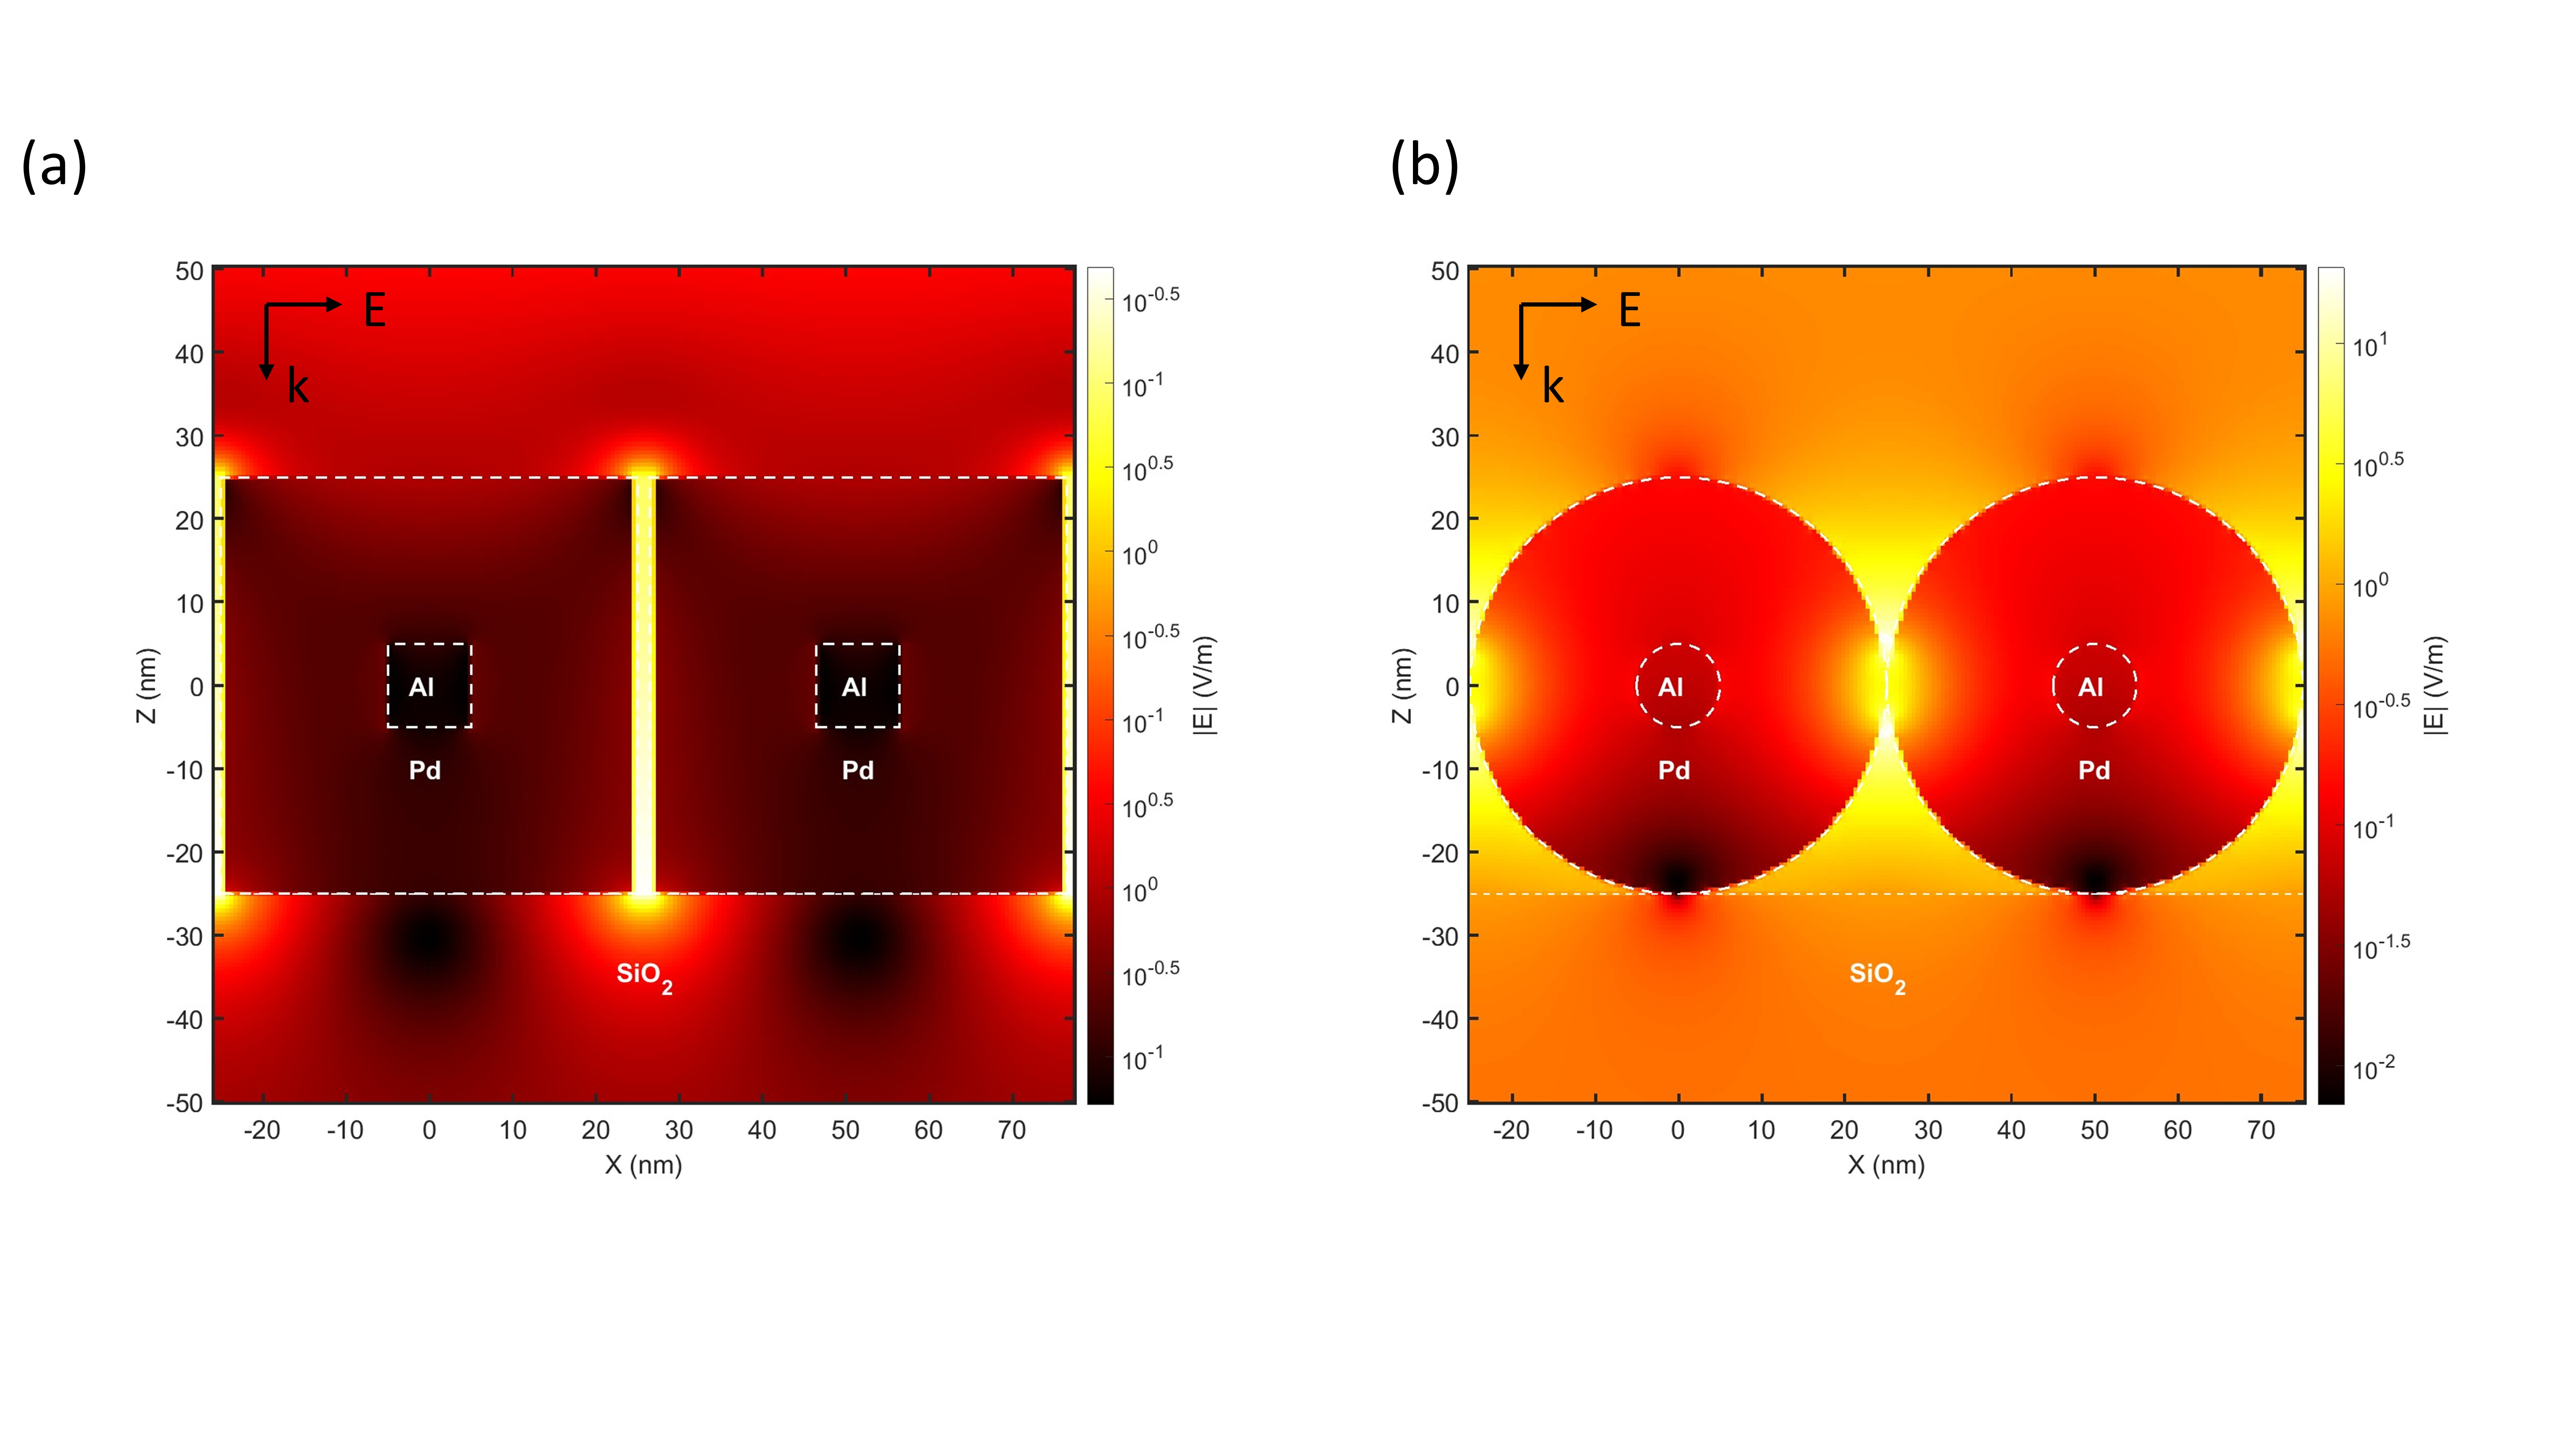
\includegraphics[width=80mm]{Efield_coreshell.jpg}
\caption{Cross-sectional view of the electric field distribution in the x–z plane for a two-period core-shell structures. (a) Core-shell cubes (L=50nm, l=10nm, d=3nm). (b) Core-shell spheres (R=25nm, r=5nm, d=0nm).} 
\label{fig:Efield_coreshell} 
\end{figure}
% Discussion
\section{Discussion}
\indent
The optimal design is found to be a multi-layer structure consisting of Pd spheres, a TiO$_2$ spacer layer, and an Al back reflector, where the Pd spheres are in close-packed contact (i.e., just touching each other). Notably, the radius of the Pd spheres does not significantly affect the absorption performance under this configuration. When the Al layer thickness is set to 40~nm, both the total optical absorption and the internal quantum efficiency (IQE) can approach nearly 100\%.\\
\indent
Moreover, the wavelength range of effective light absorption can be tuned by adjusting the thickness of the TiO$_2$ layer and the size of the Pd spheres. A TiO$_2$ thickness below 100~nm enables high absorption and IQE over a relatively broad wavelength range, while increasing the TiO$_2$ thickness to a few hundred nanometers leads to strong but narrower absorption bands.\\
\indent
However, in the current study, we assume that all generated hot carriers contribute to the chemical reaction. In practice, only those hot carriers with energies exceeding a certain threshold can effectively drive the catalytic process. This energy threshold is typically determined by the activation barrier of the target reaction.\\
\indent
Furthermore, for core–shell structures, such as those composed of an Al core and a Pd shell, a portion of the hot carriers generated in the Al core can rapidly transfer into the Pd shell. These transferred carriers may cooperate with the hot carriers generated directly within the Pd shell to participate in the chemical reaction. This interfacial carrier transfer process should also be taken into account in future modeling and analysis.\\

% Acknowledgements
\section*{Acknowledgements}
I would like to thank Prof. Gururaj Naik for his invaluable guidance and Dr. Zhichao Li for his help throughout this project. I also appreciate the support from Dr. Yu Kee Ooi, Dr. Joseph Young and Dr. Jose Moreto throughout the course.\\

% References
\bibliographystyle{IEEEtran}
\bibliography{references}

\end{document}
